\documentclass[11pt, oneside]{article} 
\usepackage{geometry}
\geometry{letterpaper} 
\usepackage{graphicx}
	
\usepackage{amssymb}
\usepackage{amsmath}
\usepackage{parskip}
\usepackage{color}
\usepackage{hyperref}

\graphicspath{{/Users/telliott_admin/Dropbox/Tex/png/}}
% \begin{center} 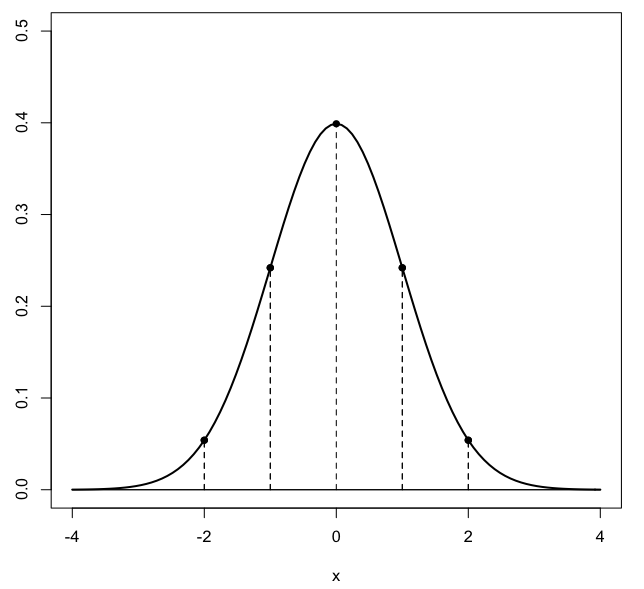
\includegraphics [scale=0.4] {gauss3.png} \end{center}

%break
\title{Derivatives of sine and cosine}
\date{}

\begin{document}
\maketitle
\Large

\subsection*{Difference quotient for sine}
The limit just obtained allows us to find the derivatives of sine and cosine.  

Set up the difference quotient for sine:
\[  \frac{\sin (x + h) - \sin x}{h} \]

Using the addition of angles formula:
\[ = \frac{\sin x \cos h + \sin h \cos x - \sin x}{h} \]
Group the terms containing $\sin x$ and $\cos x$ separately
\[ = \sin x \ \frac{(\cos h - 1)}{h} + \cos x \ \frac{\sin h}{h} \]

Evaluating the limit as $h \rightarrow 0$, the second term is
\[ \cos x \ \lim_{h \rightarrow 0} \frac{\sin h}{h} \]

We can pull $\cos x$ out of the limit, because it does not depend on $h$.  By the main result above (our "famous" limit), the limit part is equal to $1$, so the whole expression is just equal to $\cos x$.

We will show in just a minute that the first term is zero, which means that we have in the end:
\[ \frac{d}{dx} \sin x = \cos x \]
The derivative of the sine is the cosine.

\subsection*{second limit}

We massage that left-hand term from above as follows.  $\sin x$ can come out because it does not depend on $h$.  We must then evaluate
\[ \lim_{h \rightarrow 0} \ \frac{(\cos h - 1)}{h} \]
Now
\[ \frac{\cos h - 1}{h}  =  \frac{\cos h - 1}{h}  \cdot \frac{\cos h + 1}{\cos h + 1} \]

The numerator on the right is
\[ (\cos h - 1)(\cos h + 1) = \cos^2 h - 1 \]
\[ = -\sin^2 h \]
so each term on the right gets one copy of $\sin h$:
\[  - \frac{\sin h}{h} \cdot \frac{\sin h}{\cos h + 1} \]

The limit as $h \rightarrow 0$ of the first factor is equal to $1$ as we saw before, but the second one is $0/2 = 0$, so the whole thing is zero.

\[ \lim_{h \rightarrow 0} \frac{\cos h - 1}{h} = 0 \]
as promised.

\subsection*{Derivative of the cosine}

Set up the difference quotient for cosine:
\[  \frac{\cos (x + h) - \cos x}{h} \]
Using addition of angles
\[ \frac{\cos x \cos h - \sin x \sin h - \cos x}{h} \]
Grouping like terms
\[ = \cos x \ \frac{(\cos h - 1)}{h}  - \sin x \ \frac{\sin h}{h} \]

But we just showed that
\[  \lim_{h \rightarrow 0} \frac{\cos h - 1}{h} = 0 \]
so the first term is zero.  By the original limit derived above, the second term is
\[ \lim_{h \rightarrow 0} \ [ \ - \sin x \ \frac{\sin h}{h} \ ] \ = - \sin x \]

The derivative of the cosine is minus the sine.
\[ \frac{d}{dx} \ \cos x = - \sin x \]

\subsection*{Another view}
\begin{center} 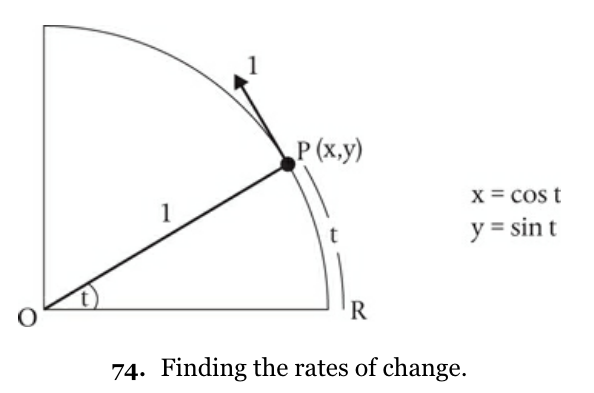
\includegraphics [scale=0.35] {Acheson_74.png} 
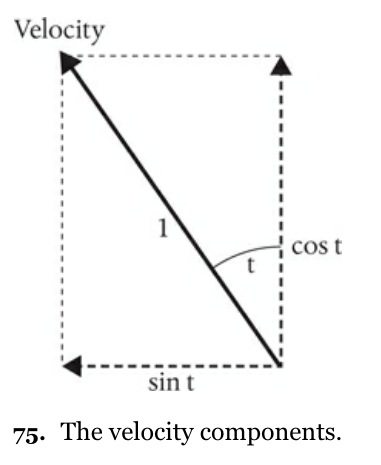
\includegraphics [scale=0.35] {Acheson_75.png} 
\end{center}
Above are two figures from Acheson:

\begin{quote}
One merit of radian measure --- together with a unit radius --- is that the distance travelled, PR, is not just proportional to the angle POR --- it is actually equal to it, and will therefore be t. 

So P travels a distance t in time t and therefore goes round and round the circle at unit speed. Its velocity at any moment is therefore 1, directed along the tangent. 

And because the tangent is perpendicular to the radius OP, this direction of motion makes an angle t with the y-axis (right panel).

Now, moving with speed 1 in the direction shown is equivalent to moving in the negative x-direction with speed sin t, at the same time as moving in the y-direction with speed cos t.
\end{quote}

That is, the $x$-component, $\cos t$, has a velocity of $- \sin t$, which is its derivative.  And the $y$-component, $\sin t$, has a velocity of $\cos t$.

\subsection*{graphs}
\begin{center} 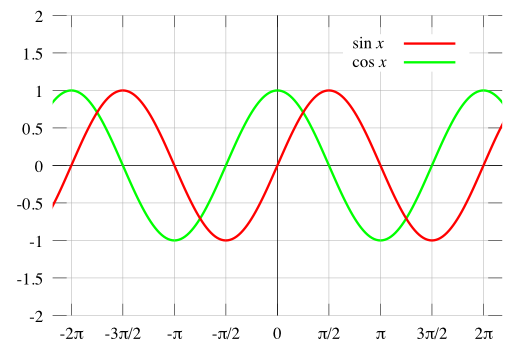
\includegraphics [scale=0.5] {sine_cosine_wikipedia.png} \end{center}

By examining the graphs of sine and cosine, we can see that the results obtained above make sense.  The maximum slope of the sine function occurs when $\theta = 0$ because $\cos \theta = \cos 0 = 1$ there, and that matches the plot.

At the top of the arc for sine, when $\theta = \pi/2$, then $\sin \theta = 1$.  The curve changes from increasing to decreasing at the very peak, and just for an instant, the slope is zero and the curve is horizontal.  The corresponding value for $\cos \theta = \cos \pi/2 = 0$.

Furthermore, the slope of sine is positive when cosine is positive, while the slope of cosine is positive when sine is negative.

\subsection*{example}
Here is a problem from Hamming that we can solve using these results.
\begin{center} 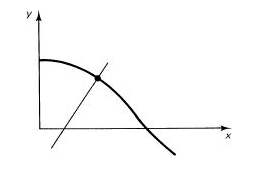
\includegraphics [scale=0.6] {y_cosx.png} \end{center}

The curve is $\cos x$ and the question is, if we form the norm (perpendicular) to the curve, does it ever pass through the origin?

The slope of the cosine is $- \sin x$.  The slope we seek is perpendicular to that, so its product must yield $-1$.  Thus $m = 1/\sin x$.

We use the point slope formula:
\[ \frac{y - y_0}{x - x_0} = \frac{1}{\sin x} \]
At the point $(x_0,y_0) = (0,0)$
\[ \frac{y}{x} = \frac{1}{\sin x} \]
But $y = \cos x$ so
\[ \sin x \cos x = x \]
\[ \frac{1}{2} \sin 2x = x \]
\[ \sin 2x = 2x \]
One solution is $(0,0)$.  Are there any more?  One way to answer this is to go back to the figure we started with where we plot $\sin x/x$:
\begin{center} 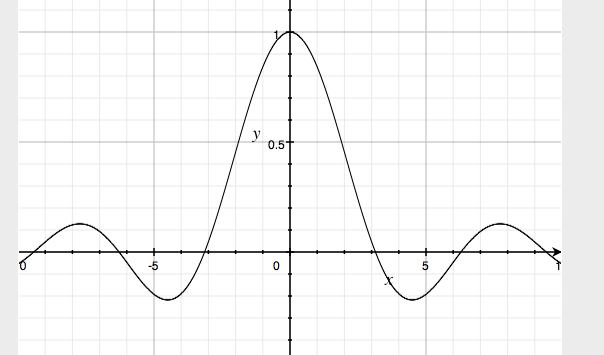
\includegraphics [scale=0.4] {sinx_over_x.png} \end{center}
No.  $\sin x = x$ happens only at $x = 0$.  In the figure, $\sin x/ x = 1$ happens only at $x=0$.

For an analytical proof, we observe that the slope of $\sin x$ is equal to $\cos x$ which is equal to $1$ at $x = 0$ and for every $x$ after that
\[ 0 < \cos x < 1, \ \ \ \ 0 < x < \frac{\pi}{2} \]
the slope of $\sin x$ is less than $1$, while the slope of $y = x$ is equal to $1$ everywhere.

The result is that the $x$ rises faster than $\sin x$ everywhere after $x = 0$.

\subsection*{Other trig functions}

We use the quotient rule, described \hyperlink{quotient_rule}{\textbf{here}}.
\[ \frac{u}{v}' = \frac{u'v - uv'}{v^2} \]

Check that we've remembered it correctly:
\[ [ \ \frac{x}{1} \ ] ' = \frac{1 \cdot 1 - x \cdot 0}{1} = 1 \]

The derivative of the tangent is
\[ \ [ \ \frac{\sin x}{\cos x} \ ]' = \frac{\cos x \cdot \cos x - \sin x (- \sin x)}{\cos^2 x} \]
\[ = \frac{1}{\cos^2 x} = \sec^2 x \]
and the secant (inverse cosine):
\[ \ [ \ \frac{1}{\cos x} \ ] ' =  \frac{-(- \sin x)}{\cos^2 x}  \]
\[ = \sec x \tan x \]

To round out the trig functions we have the cosecant and the cotangent.  They aren't seen often, except as part of a strategy of making calculus more difficult than it needs to be.

The cosecant is the inverse of the sine:
\[ \frac{d}{dx} \ \frac{1}{\sin \theta} = - \frac{1}{\sin^2 \theta} \ \cos \theta \]
\[ = - \csc \theta \cot \theta \]

And the cotangent is of course
\[  \frac{d}{dx} \ \frac{\cos \theta}{\sin \theta} = \frac{- \sin \theta \sin \theta - \cos \theta \cos \theta}{\sin^2 \theta} \]
\[ = - \frac{1}{\sin^2 \theta} = - \csc^2 \theta \]
Notice the similarity to the secant and tangent, with a change of sign as well as substitution of the cotangent and cosecant.

\subsection*{differentiation trick}
We used the sum of angles formulas (derived \hyperref[sec:sum_angles_distance]{\textbf{here}}) above.  Here are two simple tricks requiring knowledge of the derivatives that help in the finding the sum of angles.

First, if we treat $t$ as a constant and differentiate with respect to $s$ (or vice-versa) we can go between formulas pretty easily:

Start from 
\[ \cos (s + t) = \cos s \cos t - \sin s \sin t \]
Differentiate
\[ -\sin (s + t) \ ds = - \sin s \cos t \ ds - \cos s \sin t \ ds \]
\[ \sin (s + t) = \sin s \cos t + \cos s \sin t \]

Or start from 
\[ \sin (s + t) = \sin s \cos t + \cos s \sin t \]
Differentiate
\[ \cos (s + t) \ ds = \cos s \cos t \ ds - \sin s \sin t \ ds \]
\[ \cos (s + t) = \cos s \cos t - \sin s \sin t \]

\subsection*{offsets to cosine}

To rearrange the sum of angles formula above, we also need expressions for $\sin \theta$ in terms of cosine with an offset.

I find a simple approach is to take the derivative.  We have the offset to sine to find cosine as 
\[ \cos \theta = \sin (\theta + \frac{\pi}{2}) \]

the derivative is 
\[ - \sin \theta = \cos (\theta + \frac{\pi}{2}) \]
\[ \sin \theta = - \cos (\theta + \frac{\pi}{2}) = \cos (\theta - \frac{\pi}{2}) \]

\end{document}